\documentclass[border=0.125cm]{standalone}
\usepackage{tikz}
\usepackage{pgfplots}
\usepackage{graphicx}

\usetikzlibrary{decorations.pathmorphing}
\pgfplotsset{compat=newest}
\usetikzlibrary{shapes.geometric,arrows,fit,matrix,positioning}
\tikzset{main node/.style={circle,fill=black!20,draw,minimum size=3.5mm,inner sep=0pt},
         every node/.style={circle,fill=black,draw,minimum size=1mm,inner sep=0pt,label distance=-1mm},
         subtree/.style={isosceles triangle,fill=black!20,draw,minimum size=5mm,inner sep=0pt,shape border rotate=90},
         edge label/.style = {rectangle,draw=none,fill=none},
         blank edge/.style={edge from parent/.style={draw=none}},
         norm edge/.style={edge from parent/.style={black,thin,draw}},
}
\begin{document}
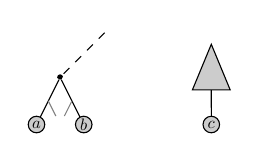
\begin{tikzpicture}[-,>=stealth', 
level 1/.style={sibling distance = 20mm},
level distance = 1cm, 
scale=0.6,
transform shape]
% \draw[help lines] (-2,0) grid (15,-15);
\node[edge label] {}
child[dashed]{
        [sibling distance = 10mm] node (1) {}
            child[solid]{
                node [main node] (2) {$a$}
            }
            child[solid]{
                node [main node] (3) {$b$}
            }
}
child[missing]{node {}}
;

\draw[gray] (-0.75,-1.5) -- (-0.91,-1.82);
\draw[gray] (-1.25,-1.5) -- (-1.09,-1.82);

\node[subtree,minimum size = 8mm] (t1_0) at (2.2,-1) {}
    child[edge from parent path = {(\tikzparentnode.south) -- (\tikzchildnode)}]{
        node[main node] (t1_1) {$c$}
    }
;

\end{tikzpicture}

\end{document}



















